\chapter{Conclusiones y trabajo futuro}
\label{sec:conclusiones}
\section{Conclusiones}

En este Trabajo Fin de Grado hemos llevado a cabo un análisis y visualización del conjunto de ceros de los \emph{polinomios ortogonales de Sobolev} cuando el producto interior incorpora derivadas de primer orden y las medidas están soportadas en la recta real o en subconjuntos compactos del plano complejo. El manuscrito ofrece un marco teórico unificado que recopila y organiza resultados clásicos y recientes sobre matrices de momentos, operadores de multiplicación de tipo Hessenberg y criterios de acotación de ceros basados en la norma del operador \(\mathcal{D}\). Esta panorámica sitúa el problema dentro de la teoría espectral moderna y facilita la comparación con otros contextos de ortogonalidad no estándar.

\textbf{Destacamos el enfoque matricial} adoptado en este trabajo, que ha permitido caracterizar los polinomios ortogonales de Sobolev a través de estructuras algebraicas que capturan completamente su comportamiento. Este enfoque ha sido fundamental para establecer conexiones entre el análisis funcional y la teoría de matrices, proporcionando herramientas computacionales robustas para el estudio de las propiedades espectrales.

Los \textbf{principales logros} de este trabajo incluyen:
\begin{itemize}
  \item Desarrollo de un marco teórico unificado para el análisis de polinomios ortogonales de Sobolev desde una perspectiva matricial.
  \item Implementación de algoritmos eficientes en \textsc{Maple} para el cálculo de matrices de Gram, ortonormalización y generación de matrices \(\mathbf{D}_n\).
  \item Creación de un sistema interactivo de visualización que permite analizar gráficamente las relaciones entre soportes, cotas teóricas y distribución de ceros.
  \item Validación numérica de las condiciones de acotación del operador \(\mathcal{D}\) en diversos contextos geométricos.
  \item Análisis pionero del comportamiento del segundo valor singular \(\sigma_{2,n}\) en operadores no secuencialmente dominados.
  \item Caracterización del efecto de los átomos en la distribución de ceros, aportando evidencia visual a una cuestión abierta.
\end{itemize}

Sobre el plano computacional, se diseñó e implementó en \textsc{Maple} un conjunto de algoritmos que, a partir de los datos de la medida, construye la matriz de Gram, ortonormaliza la base monomial, genera la familia de matrices \(\mathbf{D}_n\) y calcula tanto sus radios espectrales \(\rho(\mathbf{D}_n)\) como sus valores singulares \(\sigma_{k,n}\). A partir de esta infraestructura se elaboró un sistema interactivo de visualización que superpone los soportes de las medidas, la circunferencia de cota teórica \((|z|\le \|\mathcal{D}\|)\) y las trayectorias de los ceros al crecer el grado \(n\), facilitando la validación numérica de conjeturas y la formulación de nuevas hipótesis.

Los resultados experimentales confirman, para los casos continuos de dos circunferencias concéntricas, tangentes y disjuntas, el acotamiento uniforme de los ceros cuando el operador \(\mathcal{D}\) es acotado, reproduciendo y extendiendo los ejemplos existentes en la literatura. Por primera vez se analiza de forma sistemática el comportamiento del segundo valor singular \(\sigma_{2,n}\) en situaciones donde el operador no es secuencialmente dominado, observándose su convergencia hacia el radio máximo del soporte combinado y sugiriendo refinamientos en las cotas espectrales actuales. En el caso discreto —una medida continua perturbada por un átomo— se pone de manifiesto que la presencia del átomo fuera del disco de la medida base provoca la pérdida de acotación y la fuga de algunos ceros, aportando evidencia visual a una cuestión hasta ahora abierta.

\textbf{Contribuciones originales:}
\begin{itemize}
  \item Criterios gráficos basados en diagramas \((\rho(\mathbf{D}_n),\sigma_{2,n})\) para diagnosticar la acotación de \(\mathcal{D}\).
  \item Conjetura sobre la convergencia de \(\rho(\mathbf{D}_n)\) al radio de la envolvente convexa del soporte para productos Sobolev compacto-compacto.
  \item Conjetura sobre la convergencia de \(\sigma_{2,n}\) al máximo módulo de los puntos de soporte cuando \(\|\mathcal{D}\|=\infty\).
  \item Repositorio de casos de prueba que garantiza la reproducibilidad de los resultados.
\end{itemize}

En conjunto, el trabajo integra teoría, experimentación computacional y visualización interactiva, aportando nuevas evidencias y herramientas que favorecen la exploración de los polinomios ortogonales de Sobolev en contexto poco estudiados. Consideramos que estas contribuciones no sólo consolidan resultados previos, sino que abren vías prometedoras hacia una comprensión más profunda de la interacción entre la geometría del soporte, la estructura del producto de Sobolev y el espectro del operador de multiplicación.

Para concluir, cabe destacar que los experimentos presentados se han realizado en casos concretos de Sobolev involucrando intervalos, circunferencias y átomos. Sin embargo, los resultados obtenidos y la metodología desarrollada permiten vislumbrar generalizaciones naturales al caso de productos Sobolev asociados a medidas más generales, e incluso extenderse al contexto de \textbf{productos Sobolev matriciales}, como se esquematiza en el siguiente diagrama. Esta estructura jerárquica ilustra cómo los casos particulares estudiados se insertan en un marco teórico más amplio, proporcionando una base sólida para futuras investigaciones que busquen generalizar los resultados a contextos de mayor complejidad analítica.

\[
  \boxed{\!\!
    \begin{array}{c}
      %--- Producto de Sobolev matricial -----------------------------
      \displaystyle
      \langle p(z),q(z)\rangle_{\textbf{M}_S}
      =\langle p(z),q(z)\rangle_{\textbf{M}_1}
      +\langle p'(z),q'(z)\rangle_{\textbf{M}_2}  % definición matricial
      \\[6pt]                            % ← ajusta a gusto
      %--- Producto de Sobolev en medidas ----------------------------
      \boxed{\!\!
        \begin{array}{c}
          \displaystyle
          \langle p,q\rangle_{S}
          =\int_{\mathbb{C}} p(z)\,q(z)\,d\mu_1(z)
          +\int_{\mathbb{C}} p'(z)\,q'(z)\,d\mu_2(z)   % definición con medidas
          \\[6pt]
          %--- Sobolev  ----------------------------------------------
          \boxed{\!\!
            \begin{array}{c}
              \textbf{Sobolev} \\[4pt]
              \boxed{\text{Real}}\quad
              \boxed{\text{Circunferencia}}
            \end{array}
          }%
        \end{array}
      }%
    \end{array}
  }\!
\]

\section{Reflexión personal}

Al cursar la asignatura de Análisis Funcional y aprender sobre los espacios de Sobolev, este estudio me intrigó desde el primer momento en que me lo comentaron. Los resultados obtenidos a lo largo del trabajo me han sorprendido y, sinceramente, me he quedado con ganas de profundizar aún más en este campo.

Este TFG muestra perfectamente la esencia del Grado en Matemáticas e Informática. A diferencia de otros dobles grados duales, esta titulación busca constantemente puntos de convergencia entre ambas disciplinas. El presente trabajo, fundamentado en teoría matemática y desarrollado mediante implementaciones computacionales, ejemplifica esta intersección de manera notable. Evidencia claramente la profunda interrelación entre matemáticas e informática, mostrando cómo cada disciplina potencia a la otra para generar conocimiento innovador. La experiencia de traducir conceptos matemáticos abstractos a modelos computacionales, para luego explorarlos y validarlos mediante algoritmos, ha sido extraordinariamente formativa y refleja fielmente las competencias adquiridas durante mis estudios.

\section{Trabajos Futuros}

El presente TFG abre diversos frentes de investigación que, de abordarse con mayor profundidad, podrían consolidar y ampliar los resultados obtenidos. A continuación se describen varias líneas prioritarias, agrupadas según su naturaleza teórica, computacional y aplicada, pero sin perder de vista las ideas nucleares ya esbozadas en el texto.

\emph{Productos Sobolev de orden superior \((N>1)\).}
Un paso natural es incorporar derivadas de segundo y tercer orden en el producto interior. Continuar con el análisis de los valores singulares siguientes ($\sigma_{3,n}, \sigma_{4,n},...$), como se ilustrará en los ejemplos posteriores.

\emph{Leyes de distribución de ceros.}
Derivar distribuciones límite (tipo medida de equilibrio) para los ceros en distintos regímenes de soportes y pesos Sobolev proporcionaría una analogía con la Ley de Zeros de Ullman-Stahl en la ortogonalidad estándar.

\emph{Convergencia del autovalor máximo.}
Investigar la convergencia del autovalor que determina $\rho(\mathbf{D}_n)$, verificando si el autovalor que determina el radio espectral converge.

\emph{Átomos bpe como caso secuencialmente dominado.}
Finalmente, se profundizará en el estudio de los átomos, utilizando como base los trabajos de Gonzalo y Escribano sobre la secuencialidad matricial en el caso de productos de Sobolev con átomos.

\textbf{Ejemplo 1.}
$\langle p(t),q(t) \rangle_{S}=\int_{0}^{10} p(t)q(t)\, dt + \int_{30}^{40} p'(t)q'(t) \, dt + \int_{60}^{70} p''(t)q''(t) \, dt$

\begin{center}
  \begin{tabular}{cc}
    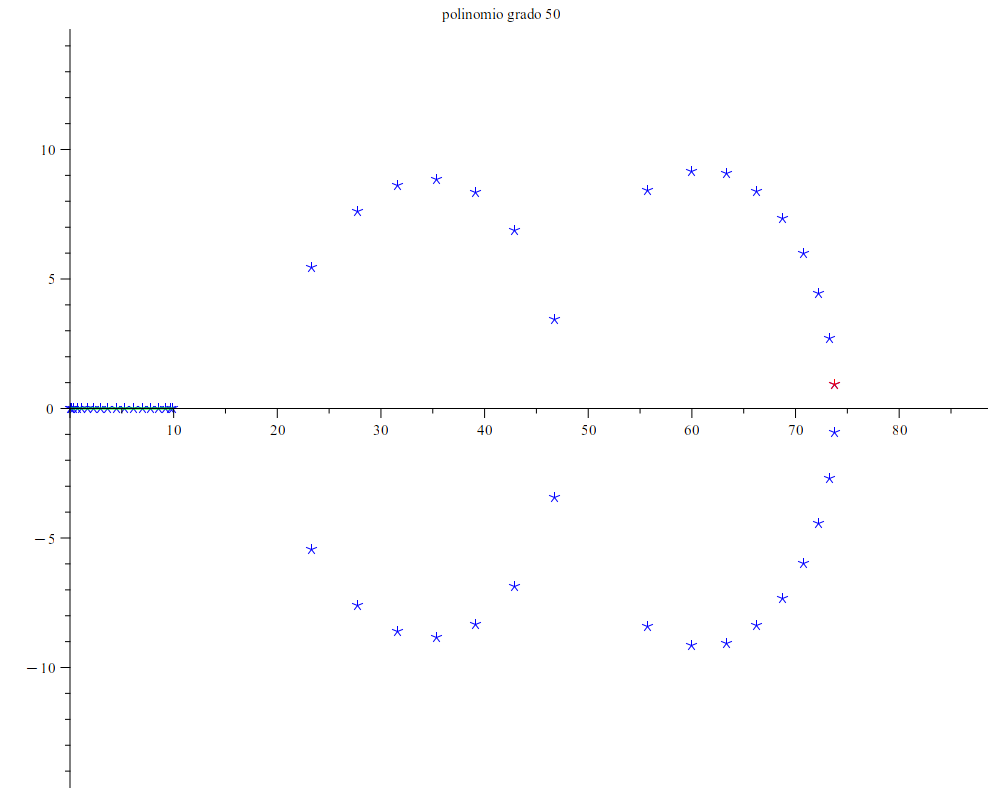
\includegraphics[width=0.45\textwidth]{include/a0b10c30d40e60f70_zero.png} &
    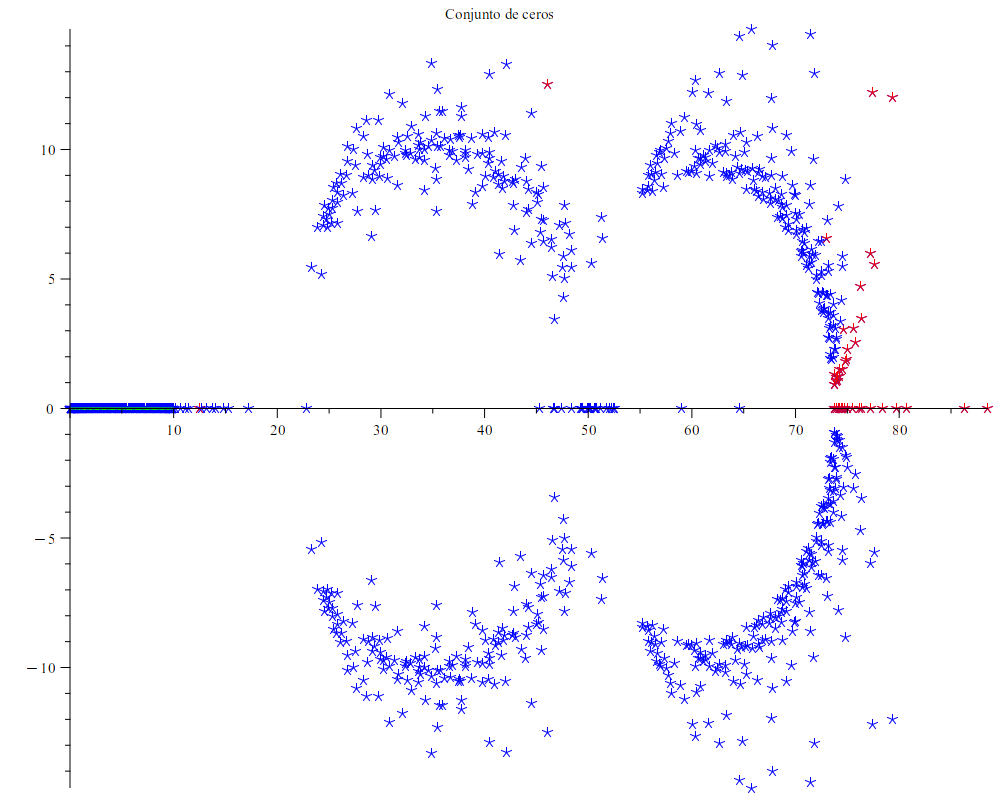
\includegraphics[width=0.45\textwidth]{include/a0b10c30d40e60f70_zeros.png}  \\
  \end{tabular}
  \begin{minipage}[b]{0.45\textwidth}
    \begin{enumerate}
      \item $\sigma_{1,70}=4.939\times10^{8}$
      \item $\sigma_{2,70}=1.847\times10^{8}$
      \item $\sigma_{3,70}=69.956$
      \item $R = 70$
      \item $ \rho(\mathbf{D}_{70})=73.791$
      \item $\max\{\rho(\mathbf{D}_{n})\}_{n=0}^{70}=88.570$
    \end{enumerate}
  \end{minipage}
\end{center}

\textbf{Ejemplo 2.}
$\langle p(t),q(t) \rangle_{S}=\int_{0}^{10} p(t)q(t)\, dt + \int_{30}^{40} p'(t)q'(t) \, dt + p''(0) c''(0) \, dt$

\begin{center}
  \begin{tabular}{cc}
    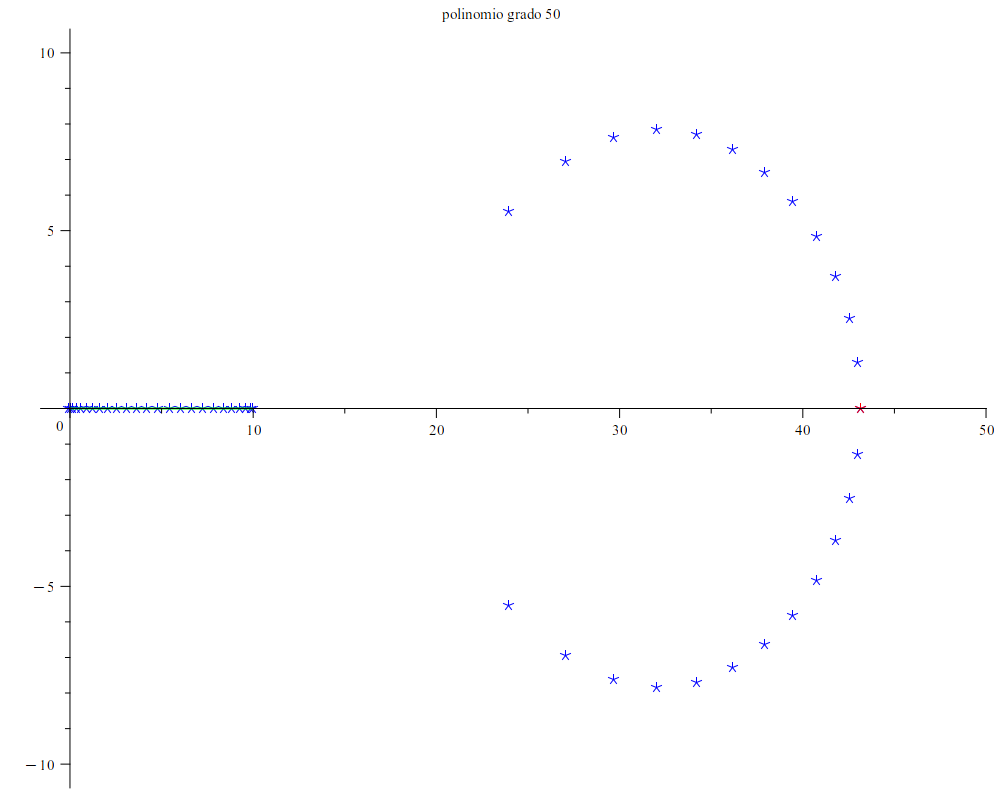
\includegraphics[width=0.45\textwidth]{include/a0b10c30d40t0_zero.png} &
    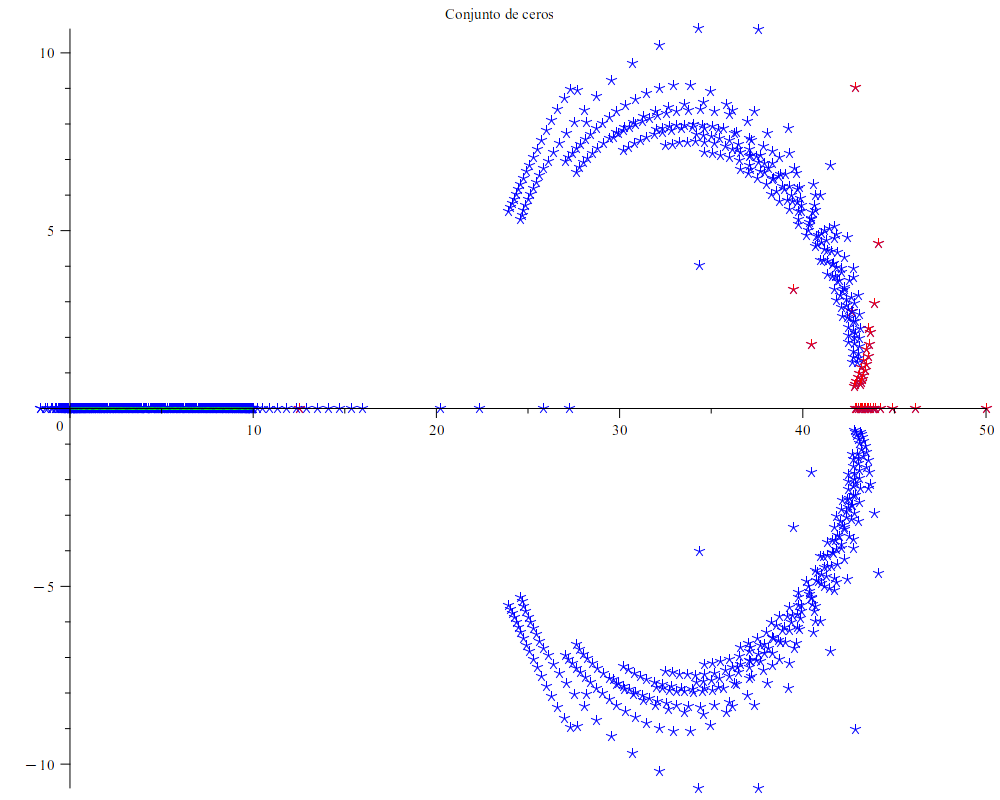
\includegraphics[width=0.45\textwidth]{include/a0b10c30d40t0_zeros.png}  \\
  \end{tabular}
  \begin{minipage}[b]{0.45\textwidth}
    \begin{enumerate}
      \item $\sigma_{1,70}=1.521\times10^{12}$
      \item $\sigma_{2,70}=212.771$
      \item $\sigma_{3,70}=39.976$
      \item $R = 40$
      \item $ \rho(\mathbf{D}_{70})=43.136$
      \item $\max\{\rho(\mathbf{D}_{n})\}_{n=0}^{70}=50.046$
    \end{enumerate}
  \end{minipage}
\end{center}

Como se puede observar en los ejemplos, $\sigma_{1,n} = \infty$ y $\sigma_{2,n} = \infty $ , mientras que $\sigma_{3,n} = R < \infty$.

En resumen, estas líneas de investigación futura prometen extender el alcance y la profundidad de los resultados obtenidos en este TFG, estableciendo conexiones más sólidas entre la teoría espectral y los polinomios ortogonales de Sobolev. El marco teórico desarrollado, junto con las herramientas computacionales implementadas, proporciona una base robusta desde la cual abordar estos desafíos, contribuyendo así a una comprensión más completa de la interacción entre estructura algebraica, propiedades espectrales y comportamiento asintótico en sistemas polinomiales con derivadas.




